\section{Tickets}
\label{sec:tickets}

In the HOPR protocol, nodes that have staked funds within a payment channel can
issue tickets that are used for payment to other nodes. Tickets are used for
\nameref{sec:probabilisticpayments}; every ticket is bound to a specific payment
channel and cannot be spent elsewhere. Tickets are redeemable at most once and
lose their value when the associated payment channel is closed or when the commitment is reset. A
commitment is a secret on-chain value used to verify whether a ticket is
a winner or not when an attempt is made to redeem it.

\subsection{Ticket Issuance}

A ticket can be issued when two nodes have established a payment channel with
each other. By definition this means at least one of them has staked HOPR tokens.

The ticket issuer $A$ (who could also be the packet creator) selects the
winning probability of the ticket and the relay fee to use and sets the amount to:
$$\sigma=\dfrac{L\times F}{P_w}$$
where $\sigma$ is the amount of HOPR tokens set in the ticket, $L$ is the path
length, $F$ is the relay fee, and $P_w$ is the ticket's winning probability.

$A$ issues a ticket for the next downstream node.
The challenge is given together with the routing information by the packet.

$A$ does not know whether the ticket is a winner or not.
    
$A$ sets the content of the ticket to: $$t=(R,\sigma,P_w,\alpha,I,T_c,\zeta),$$ where $t$ has the following components, in addition to those already defined above:
\begin{itemize}
\item \textbf{Recipient's Ethereum address $R$}: a unique identifier derived from the ticket recipient's public key.
\item \textbf{Ticket epoch $\alpha$}: used as a mechanism to prevent cheating by turning non-winning tickets into winning ones. This is done by increasing the value of $\alpha$ whenever a node resets a commitment, which helps keep track of updates to the on-chain commitments and invalidates tickets from earlier epochs.
\item \textbf{Ticket index $I$}: set by the ticket issuer and increases with every issued ticket. The recipient verifies that the index increases with every packet and drops any packets where this is not the case. Redeeming a ticket with index $n$ invalidates all tickets with index $I<n$, hence the relayer has a strong incentive to not accept tickets with an unchanged index.
\item \textbf{Ticket challenge $T_c$}: set by the ticket issuer and used to check whether a ticket is redeemable before the packet is been relayed. If it is not redeemable, the packet is dropped.
\item \textbf{Channel epoch $\zeta$}: used to give each incarnation of the payment channel a new identifier such that tickets issued for previous instances of the channel become invalid once a channel is reopened ($\alpha$'s count restarts again). This is due to the fact that $\zeta$ increments whenever a closed channel is (re)opened.
\end{itemize}

$A$ then signs the ticket with its private key and sends $T = (t, Sig_I(t))$ to the recipient together with a mixnet packet.
    \begin{comment}


    \\\textbf{ChainId $c_{Id}$:} The channel identifier which is defined by the ticket issuer in order to determine which channel will be used between issuer and recipient. For example, tickets that are valid on xDAI are not valid on Ethereum.
    \\\textbf{Tag $\tau$} is given as a constant and depends on the utilized blockchain. It is used to distinguish HOPR tickets from others with the same structure that are meant for different payment channels and invalidates their usage in HOPR.
    \\\textbf{Version $V$} is given as a constant and depends on the utilized blockchain. It is used to invalidate tickets that were issued for previous versions of HOPR from being used in future iterations of the protocol.

\end{comment}

    \begin{figure}[H]
        \centering
        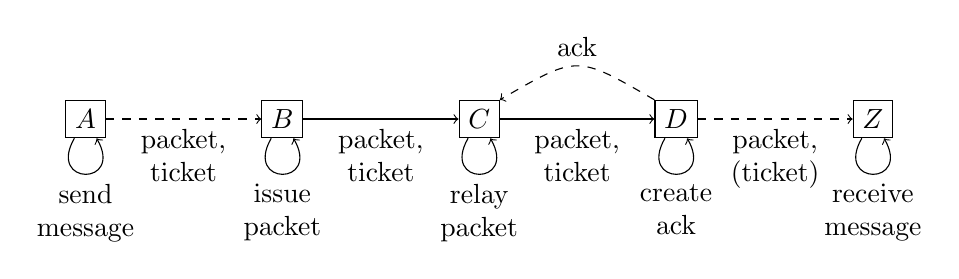
\begin{tikzpicture}[auto]
            \draw (0,0) node (a) [rectangle,draw] {$A$};
            \draw (2.5,0) node (b) [rectangle,draw] {$B$};
            \draw (5,0) node (c) [rectangle,draw] {$C$};
            \draw (7.5,0) node (d) [rectangle,draw] {$D$};
            \draw (10,0) node (z) [rectangle,draw] {$Z$};

            \draw [->,draw,dashed] (a.east) to node [align=center,below] {packet,\\ticket} (b.west);
            \draw [->,draw] (b.east) to node [align=center,below] {packet,\\ticket} (c.west);
            \draw [->,draw] (c.east) to node [align=center,below] {packet,\\ticket} (d.west);
            \draw [->,draw,dashed] (d.east) to node [align=center,below] {packet,\\(ticket)}  (z.west);

            \path[->] (a) edge [out=-120,in=-60,distance=2em,below] node [align=center] {send\\message}  (a);    % \draw 
            \path[->] (b) edge [out=-120,in=-60,distance=2em,below] node [align=center] {issue\\packet}  (b);    % \draw 
            \path[->] (c) edge [out=-120,in=-60,distance=2em,below] node [align=center] {relay\\packet}  (c);    % \draw 
            \path[->] (d) edge [out=-120,in=-60,distance=2em,below] node [align=center] {create\\ack}  (d);    % \draw 
            \path[->] (z) edge [out=-120,in=-60,distance=2em,below] node [align=center] {receive\\message}  (z);    % \draw 

            \path[->,draw,looseness=1.5,dashed,bend right] (d.north west) to [above] node {ack} (c.north east);
        \end{tikzpicture}    \caption{Ticket workflow}
        \label{fig:Ticket worklow}
    \end{figure}


\subsection{Ticket Validation}

Tickets are received together with packets. To this end, the recipient and the next downstream node share a secret, $s$, whose key shares $s_i$ and $s_{i+1}$ are derivable by those nodes. Ticket validation requires the following steps:

 \textbf{Validate response} Once $A$ receives $s_{i+1}^{(1)}$ from $B$ via secret sharing, it can compute $$r_i=s_i^{(0)}+s_{i+1}^{(1)}$$ where $r_i$ is the response $r$ at iteration $i$ such that it verifies
$$r_i*G=T_{c_i}$$
\\\textbf{Validate hint} Once the recipient transforms the packet, it can compute $s_i$. The recipient can now also extract the routing information from the packet.
This includes a hint to the value $s_{i+1}$, given as $$H_i=s_{i+1}^{(1)}*G,$$ which is stored in the Sphinx packet header.

The unacknowledged ticket is stored in the database under the hint to the promised value to ensure the acknowledgement can be later linked to the unacknowledged ticket.

Together with $s_i^{(0)}$, the node can verify that $$T_{c_i}=s_i^{(0)}*G+H_i$$ with $$s_i^{(0)}*G+H_i=s_i^{(0)}*G+s_{i+1}^{(1)}*G=(s_i^{(0)}+s_{i+1}^{(1)})*G$$
This allows the recipient to verify that the promised value $s_{i+1}^{(1)}$ indeed leads to a solution of the challenge given in the ticket. If this is not the case, the node should drop the packet. Without this check, the sender could intentionally create false challenges which lead to unredeemable tickets.


\subsection{Ticket Redemption}

In order to unlock a ticket, the recipient node stores the ticket within its database until it receives an acknowledgement containing $s_{i+1}$ from the next downstream node. HOPR uses acknowledgements to prove the correct transformation of mixnet packets as well as their delivery to the next downstream node.

The challenge can be computed from the acknowledgement as $T_{c_i}=Ack_i*G$. The node checks the following in order to redeem its ticket:
\begin{itemize}
\item \textbf{Stored ticket} Once the node receives an acknowledgement, it checks whether it is storing an unacknowledged ticket corresponding to the received acknowledgement. If it does not, the node should drop the acknowledgement.

 The node then computes the response to the challenge (also referred to as the \textit{proof of relay secret}) given in the ticket as $$r_i=(s_i^{(0)}+s_{i+1}^{(1)})*G$$
\item  \textbf{Sufficient challenge information} The node checks whether the information gained from the packet transformation is sufficient to fulfil the challenge sent along with the ticket, $$r_i*G=T_{c_i}$$
The node then replies with an acknowledgement which includes a response to the challenge. If this is not the case, the node should drop the packet.
\end{itemize}

Both the node and the smart contract then perform the following checks: 

\begin{itemize}
\item \textbf{Channel existence} The node checks that the appropriate channel \textbf{exists} and is \textbf{open} or \textbf{pending to close}. If these checks do not pass, the node should drop the packet and the smart contract check will revert. To prevent metadata leakage, the check happens locally rather than on-chain using the blockchain indexer. If the node has no record of the channel or considers the channel to be in a state different from \textbf{open} or \textbf{pending to close}, the ticket is dropped and receipt of the accompanying packet is rejected.
\item \textbf{Commitment value check} Additionally, the node and the smart contract retrieve the next commitment value, $comm_{i-1}$. They then check that this value is not empty and that the commitment is the opening of the next commitment as follows:
$$ comm_{i-1} != 0 \; and \; comm_{i}=h(comm_{i-1})$$
\item \textbf{Commitment verification} The node then verifies that $r_i$ and $comm_{i-1}$ lead to a winning ticket.
This is the case if $$h(t_h, comm_{i-1}, r_i) <P_w$$ where $t_h=h(t)$ is the ticket hash. The values are first ABI encoded, then hashed using keccak256 and last but not least converted to uint256.

If the check is not valid, the node should drop the packet.
The final recipient of the packet does not receive a ticket because packet reception is not incentivized by the HOPR protocol.
\item \textbf{Issuer identity} The ticket signer must be same as the ticket issuer. Both node and smart contract verify if the public key associated to the private key used to sign $$T= (t, Sig_I(t))$$ is the issuer's public key. The packet is dropped if this test fails.
\item \textbf{Prior redemption} The ticket must not have been already redeemed and the ticket index must be strictly greater than the current value in the smart contract (replay protection).
     $$I_c <I$$ where $I_c$ is the current value in the smart contract and $I$ is the ticket index.
\item \textbf{Valid ticket amount} The amount of ticket must be greater than 0: $$\sigma>0$$ where $\sigma$ is the ticket amount.
\item \textbf{Liquidity check} The channel must have enough funds to cover the value transfer for the ticket: $$ C_b>\sigma$$ where $C_b$ is the channel balance.
\end{itemize}

Finally, the smart contract also performs an epoch check:
\begin{itemize}
\item \textbf{Epoch check} The ticket epoch, $\alpha$, and channel epoch, $\zeta$, must be equal to the current values in the smart contract $$\alpha=\alpha_c \;\; and \;\; \zeta=\zeta_c$$
where $\alpha_c$ and $\zeta_c$ represent the current values in the smart contract.
\end{itemize}
